%************************************************
\chapter*{Summary}
\chaptermark{Summary} %otherwise gets it wrong? Like for Introduction
\label{pt:summary}
In this thesis, we have studied how spatial inhomogeneities can prohibit a system's thermalization at least on short and intermediate timescales. In \autoref{pt:spatial-disorder}, we studied closed quantum systems featuring power-law interactions and demonstrated the presence of an emergent integrability following the structure of MBL. This feature appeared to be robust using numerical finite size scaling and also experimental data showed clear signatures of its consequences even in a critical case where $\alpha=d=3$. While the existence of MBL as a true thermodynamic phase is hotly debated, its core concept, i.e. the disorder-induced emergent integrability, proved to be a very useful tool to understand the behavior of real-world experiments. Whether or not this apparent localization persists to infinite times and infinite system size can perhaps be answered by generalizing the perturbative RSRG procedure to higher orders but this is beyond the scope of this work.

Then, in \autoref{pt:floquet}, we considered periodically driven systems and discerned the intricate interplay of driving and non-trivial, quasi-conserved quantities caused by spatial inhomogeneity. The key signature of these conservation laws manifests as long-lived oscillations that have a frequency that is an integer multiple of the driving frequency. However, we have seen that the details of the conservation laws and the connected symmetries have a strong influence on the stability of the dynamics.
Thus, the microscopic structure of the system imprints on its macroscopic dynamics allowing for novel physics out-of-equilibrium.

More generally, we have seen that the absence of thermalization often comes with additional structure.
Hence, even though out-of-equilibrium states are, per definitionem, not amenable to a thermal description, all is it not lost. For the systems studied here, effective conservation laws could be identified and subsequently exploited to gain insight into the systems' dynamics.

%We considered both closed quantum systems with power-law interactions as well as periodically driven systems with nearest-neighbor interactions and detailed how the spatial disorder leads to non-trivial, quasi-conserved, quantities. These effective conservation laws allow for making predictions about the systems recovering predictive power even in the absence of thermalization.

%\FIXME{Expand first paragraph}
%
%Additionally, by studying power-law interaction models subject to spatial disorder in Part \ref{pt:spatial-disorder}, we demonstrated that there is an emergent integrability similar to MBL. This featured appeared to be robust using numerical finite size scaling and the experimental data showed clear signatures of its consequences even in a critical case where $\alpha=d=3$. While the existence of MBL as a true thermodynamic phase is hotly debated, its core concept, i.e. the disorder-induced emergent integrability, proofed to be a very useful tool understand the behavior of real-world experiments. 

%So while many systems, classical or quantum, thermalize quickly, there are exceptions to this rule when systems are subjected to disorder. These disordered systems evade a thermal description for long times or perhaps indefinitely thus preventing the approach by statistical mechanics. For the systems studied here, the absence of thermalization was caused by effective conservation laws which instead could be exploited to gain insight into the systems' dynamics.

Speaking in terms of coffee: In a latte, the milk and coffee always intermix quickly. However, if the milk is strongly
disordered, i.e. frothy, then it will not mix well into the coffee even if stirred. However the resulting macchiato is not much harder to describe than the latte. It just features some additional structure.
At least in this regard, quantum systems are akin to coffee.

\begin{figure}[hbt]
	\centering
	\hfil
	\raisebox{-0.5\height}{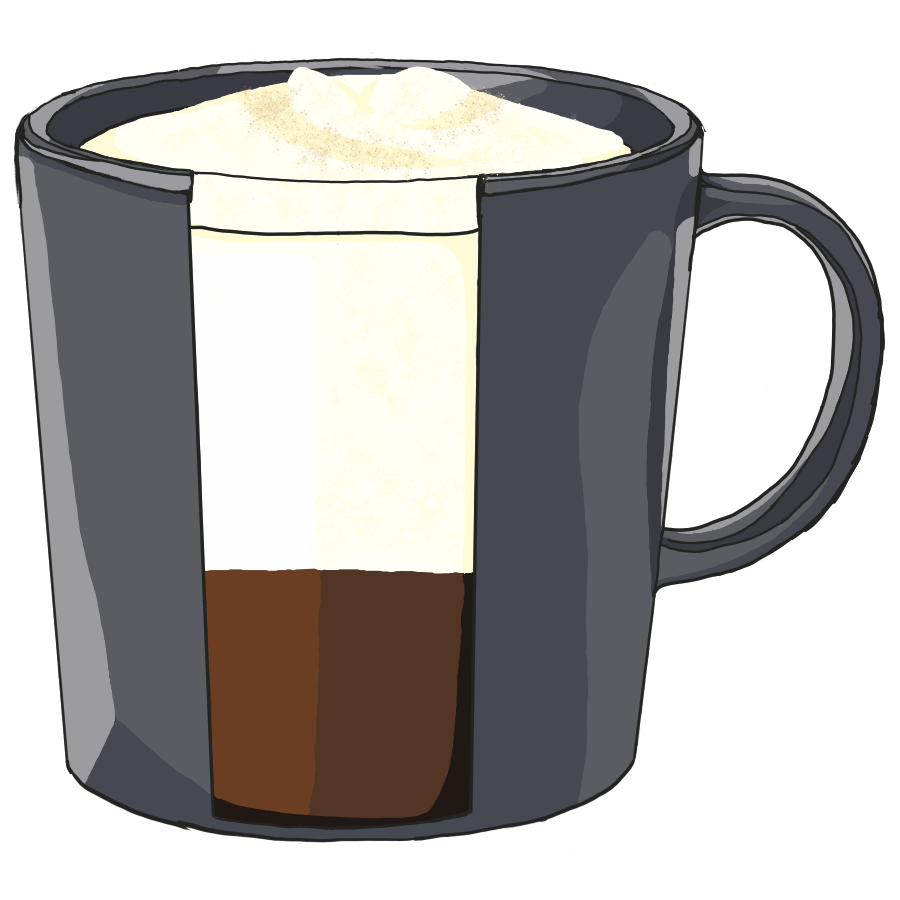
\includegraphics[width=0.3\textwidth]{gfx/intro/Kaffeetasse_Q1.png}}
	\hfil
	\raisebox{-0.5\height}{\scalebox{4}{$\longrightarrow$}}
	\hfil
	\raisebox{-0.5\height}{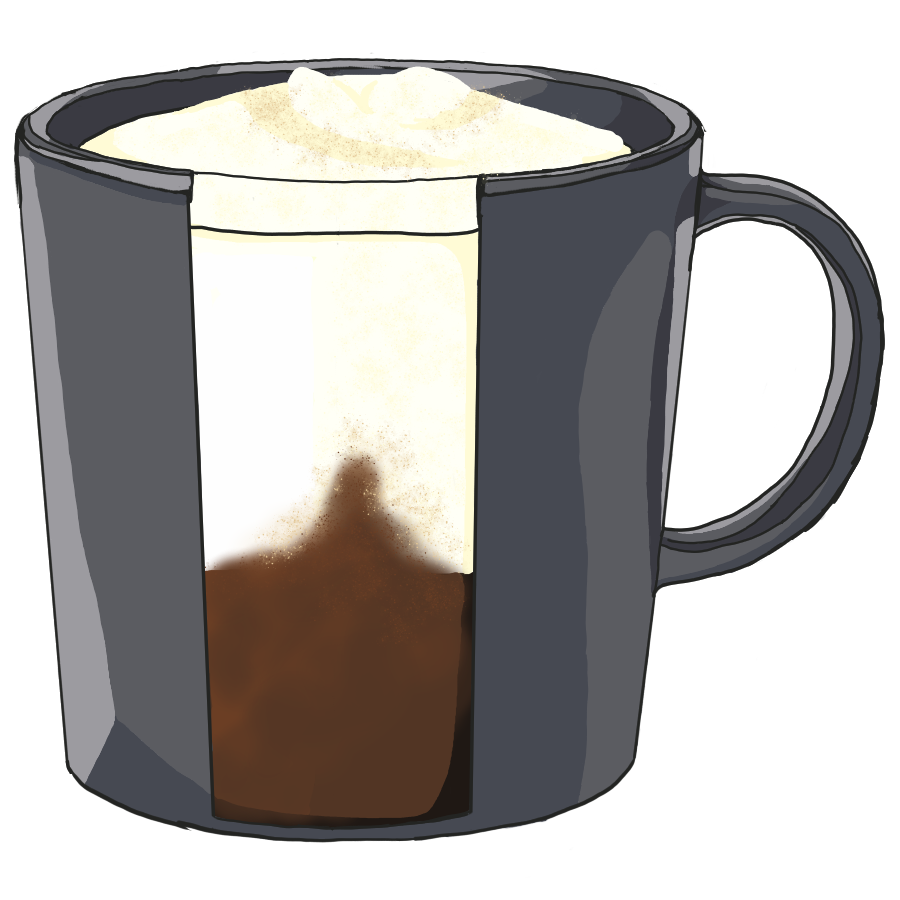
\includegraphics[width=0.3\textwidth]{gfx/intro/Kaffeetasse_Q2.png}}
	\hfil
	\caption{Localization exemplified by a macchiato.}
	\label{fig:localized-macciato}
\end{figure}
